\documentclass[notes,serif]{beamer}
\usepackage{graphicx}
\usepackage{url}
\usepackage{clrscode}
\usepackage{amssymb,amsmath}

% You should run 'pdflatex' TWICE, because of TOC issues.

\mode<presentation>
{
  % A tip: pick a theme you like first, and THEN modify the color theme, and then add math content.
  % Warsaw is the theme selected by default in Beamer's installation sample files.

  %%%%%%%%%%%%%%%%%%%%%%%%%%%% THEME
  %\usetheme{AnnArbor}
  %\usetheme{Antibes}
  %\usetheme{Bergen}
  %\usetheme{Berkeley}
  %\usetheme{Berlin}
  %\usetheme{Boadilla}
  %\usetheme{boxes}
  %\usetheme{CambridgeUS}
  %\usetheme{Copenhagen}
  %\usetheme{Darmstadt}
  %\usetheme{default}
  %\usetheme{Dresden}
  %\usetheme{Frankfurt}
  %\usetheme{Goettingen}
  %\usetheme{Hannover}
  %\usetheme{Ilmenau}
  %\usetheme{JuanLesPins}
  %\usetheme{Luebeck}
  %\usetheme{Madrid}
  %\usetheme{Malmoe}
  %\usetheme{Marburg}
  %\usetheme{Montpellier}
  %\usetheme{PaloAlto}
  %\usetheme{Pittsburgh}
  %\usetheme{Rochester}
  %\usetheme{Singapore}
  %\usetheme{Szeged}
  \usetheme{Warsaw}

  %%%%%%%%%%%%%%%%%%%%%%%%%%%% COLOR THEME
  %\usecolortheme{albatross}
  %\usecolortheme{beetle}
  %\usecolortheme{crane}
  \usecolortheme{default}
  %\usecolortheme{dolphin}
  %\usecolortheme{dove}
  %\usecolortheme{fly}
  %\usecolortheme{lily}
  %\usecolortheme{orchid}
  %\usecolortheme{rose}
  %\usecolortheme{seagull}
  %\usecolortheme{seahorse}
  %\usecolortheme{sidebartab}
  %\usecolortheme{structure}
  %\usecolortheme{whale}

  %%%%%%%%%%%%%%%%%%%%%%%%%%%% OUTER THEME
  %\useoutertheme{default}
  %\useoutertheme{infolines}
  %\useoutertheme{miniframes}
  %\useoutertheme{shadow}
  %\useoutertheme{sidebar}
  %\useoutertheme{smoothbars}
  %\useoutertheme{smoothtree}
  %\useoutertheme{split}
  %\useoutertheme{tree}

  %%%%%%%%%%%%%%%%%%%%%%%%%%%% INNER THEME
  %\useinnertheme{circles}
  %\useinnertheme{default}
  %\useinnertheme{inmargin}
  %\useinnertheme{rectangles}
  %\useinnertheme{rounded}

  %%%%%%%%%%%%%%%%%%%%%%%%%%%%%%%%%%%

%  \setbeamercovered{transparent} % or whatever (possibly just delete it)
  \setbeamercovered{invisible} % or whatever (possibly just delete it)
  % To change behavior of \uncover from graying out to totally invisible, can change \setbeamercovered to invisible instead of transparent. apparently there are also 'dynamic' modes that make the amount of graying depend on how long it'll take until the thing is uncovered.

}


% Get rid of nav bar
\beamertemplatenavigationsymbolsempty

% Use short top
%\usepackage[headheight=12pt,footheight=12pt]{beamerthemeboxes}
%\addheadboxtemplate{\color{black}}{
%\hskip0.3cm
%\color{white}
%\insertshortauthor \ \ \ \
%\insertframenumber \ \ \ \ \ \ \
%\insertsection \ \ \ \ \ \ \ \ \ \ \ \ \ \ \ \ \  \insertsubsection
%\hskip0.3cm}
%\addheadboxtemplate{\color{black}}{
%\color{white}
%\ \ \ \
%\insertsection
%}
%\addheadboxtemplate{\color{black}}{
%\color{white}
%\ \ \ \
%\insertsubsection
%}

% Insert frame number at bottom of the page.
\usefoottemplate{\hfil\tiny{\color{black!90}\insertframenumber}}

\usepackage[english]{babel}
\usepackage[latin1]{inputenc}

\usepackage{times}
\usepackage[T1]{fontenc}

\title{Network Programming}
\subtitle{Lecture 1---Introduction and TCP/IP}

\author{Lei Wang}

\institute{Dalian University of Technology}

%\date{Date}
\date{Nov 10, 2018}

\subject{Talks}

\def\defn#1{{\color{red} #1}}

\begin{document}

\begin{frame}
  \titlepage
\end{frame}

\begin{frame}
  \frametitle{Part 1. Introduction and TCP/IP}
  \tableofcontents
\end{frame}

\section{Introduction}
\subsection{A Simple Daytime Client}

\begin{frame}
  \frametitle{A Simple Daytime Client}
  \begin{itemize}
  \item Build Socket
  \item Establish Connection With Server
  \item Get Date
  \item Show Date
  \item Exit
  \end{itemize}
\end{frame}


\begin{frame}[containsverbatim]
\frametitle{A Simple Daytime Client - Code}

{\tiny
  \begin{verbatim}
       ...
 8     if (argc != 2)
 9         err_quit("usage: a.out <IPaddress>");

10     if ( (sockfd = socket(AF_INET, SOCK_STREAM, 0)) < 0)
11         err_sys("socket error");

12     bzero(&servaddr, sizeof(servaddr));
13     servaddr.sin_family = AF_INET;
14     servaddr.sin_port = htons(13);  /* daytime server */
15     if (inet_pton(AF_INET, argv[1], &servaddr.sin_addr) <= 0)
16         err_quit("inet_pton error for %s", argv[1]);

17     if (connect(sockfd, (SA *) &servaddr, sizeof(servaddr)) < 0)
18         err_sys("connect error");

19     while ( (n = read(sockfd, recvline, MAXLINE)) > 0) {
20         recvline[n] = 0;        /* null terminate */
21         if (fputs(recvline, stdout) == EOF)
22             err_sys("fputs error");
23     }
24     if (n < 0)
25         err_sys("read error");

26     exit(0);
27 }
  \end{verbatim}
  }
\end{frame}


\subsection{A Simple Daytime Server}

\begin{frame}
  \frametitle{A Simple Daytime Server}
  \begin{itemize}
  \item Build Socket And Listen
  \item Accept Client's Connection
  \item Send Date
  \item Release Connection
  \item Serve Next Client
  \end{itemize}
\end{frame}

\begin{frame}[containsverbatim]

\frametitle{A Simple Daytime Server - Code}
  {\tiny
  \begin{verbatim}
       ...
10     listenfd = Socket(AF_INET, SOCK_STREAM, 0);

11     bzeros(&servaddr, sizeof(servaddr));
12     servaddr.sin_family = AF_INET;
13     servaddr.sin_addr.s_addr = htonl(INADDR_ANY);
14     servaddr.sin_port = htons(13); /* daytime server */

15     Bind(listenfd, (SA *) &servaddr, sizeof(servaddr));

16     Listen(listenfd, LISTENQ);

17     for ( ; ; ) {
18         connfd = Accept(listenfd, (SA *) NULL, NULL);

19         ticks = time(NULL);
20         snprintf(buff, sizeof(buff), "%.24s\r\n", ctime(&ticks));
21         Write(connfd, buff, strlen(buff));

22         Close(connfd);
23     }
24 }
  \end{verbatim}
  }
\end{frame}

\section{The Transport Layer: TCP, UDP and SCTP}

\subsection{The Big Picture}
\begin{frame}
  \frametitle{The Big Picture}
  \begin{center}
  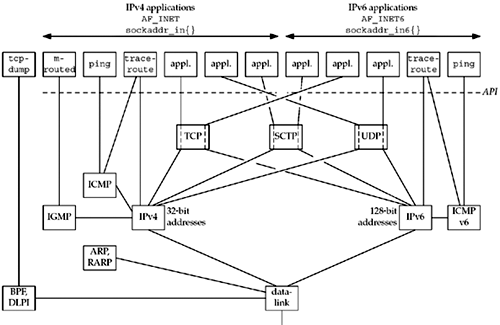
\includegraphics[width=.8\textwidth]{figs/02fig01.png}
  \end{center}
\end{frame}

\subsection{User Datagram Protocol (UDP)}
\begin{frame}
  \frametitle{User Datagram Protocol (UDP)}
  \begin{itemize}
    \item The application writes a datagram to a UDP socket, which is encapsulated as either a IPv4 of a IPv6 datagram, which is sent to its destination.
    \item UDP provides a connectionless service.
    \item Each UDP datagram has a length and we can consider a datagram as a record.
    \item RFC 768 [Postel 1980]
  \end{itemize}
\end{frame}

\subsection{Transmission Control Protocol (TCP)}
\begin{frame}
  \frametitle{Transmission Control Protocol (TCP)}
  \begin{itemize}
    \item Connection-oriented
    \item Reliable
    \item {\bf \em Sequence} the data by associating a sequence number with every byte that it sends.
    \item TCP provides {\bf \em flow control}. ---{\bf window}
    \item A TCP connection is also {\bf \em full-duplex}.
  \end{itemize}
\end{frame}

\begin{frame}
  \frametitle{TCP Connection Establishment and Termination}
  \begin{itemize}
    \item Three-Way Handshake (SYN, ACK)
    \item Four-Way Termination (FIN, ACK)
    \vskip 1em
  \end{itemize}

  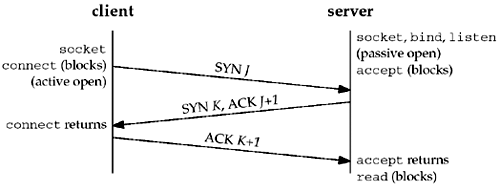
\includegraphics[height=2.5cm]{figs/02fig02.png}
  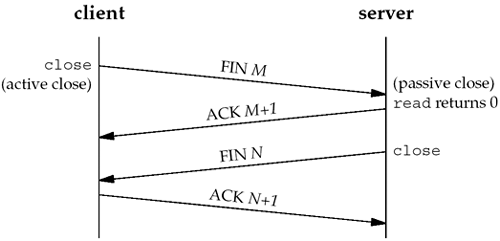
\includegraphics[height=2.5cm]{figs/02fig03.png}
\end{frame}

\begin{frame}
  \frametitle{TCP Limitations}
  \begin{itemize}
    \item TCP provides both reliable data transfer and strict order-of- transmission
    delivery of data. Some applications need reliable transfer without sequence maintenance,
    while others would be satisfied with partial ordering of the data.
    \item The stream-oriented nature of TCP is often an inconvenience.
    Applications must add their own record marking.
    \item The limited scope of TCP sockets complicates the task of providing highly-available data transfer capability using multi-homed hosts.
    \item Vulnerable to denial-of-service attacks, e.g. SYN attacks.
  \end{itemize}
  These limitations affect the performance of IP over public switched telephone networks.
\end{frame}

\subsection{Stream Control Transmission Protocol (SCTP)}
\begin{frame}
  \frametitle{Stream Control Transmission Protocol (SCTP)}
\begin{itemize}
  \item Multihoming support, where one (or both) endpoints of a connection can consist of more than one IP address, fail-over between redundant network paths.
  \item Delivery of data in chunks within independent streams.
  \item Path Selection and Monitoring.
  \item Validation and Acknowledgment mechanisms---Protects against flooding attacks and provides notification of duplicated or missing data chunks.
  \item Improved error detection suitable for jumbo Ethernet frames.
\end{itemize}
\end{frame}

\subsection{Port Numbers}
\begin{frame}
  \frametitle{Port Numbers}
    \begin{itemize}
      \item The {\bf \em well-known} ports: 0 through 1023
      \item The {\bf \em registered} ports: 1024 through 49151
      \item The {\bf \em dynamic} or {\bf \em private ports}: 49152 through 65535
    \end{itemize}
    \hspace{2em} 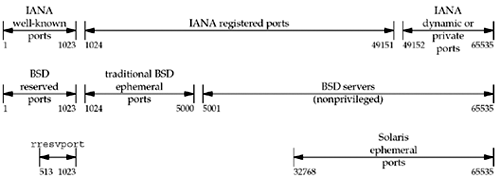
\includegraphics[height=3cm]{figs/02fig10.png}
\end{frame}

\subsection{TCP Port Numbers and Concurrent Servers}
\begin{frame}
  \frametitle{TCP Port Numbers and Concurrent Servers}
  \begin{center}
  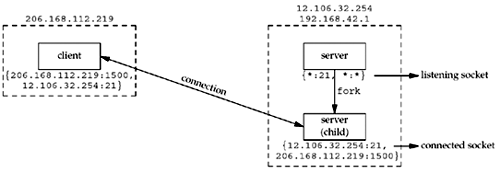
\includegraphics[height=4cm]{figs/02fig13.png}
  \end{center}
\end{frame}

\begin{frame}
  \frametitle{TCP Port Numbers and Concurrent Servers}
  \begin{center}
  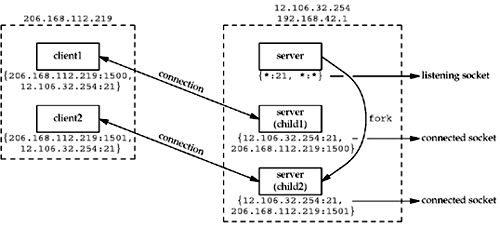
\includegraphics[height=5cm]{figs/02fig14.png}
  \end{center}
\end{frame}


\subsection{Summary}
\begin{frame}
  \frametitle{Protocol Usage by Common Internet Applications}
  \begin{center}
  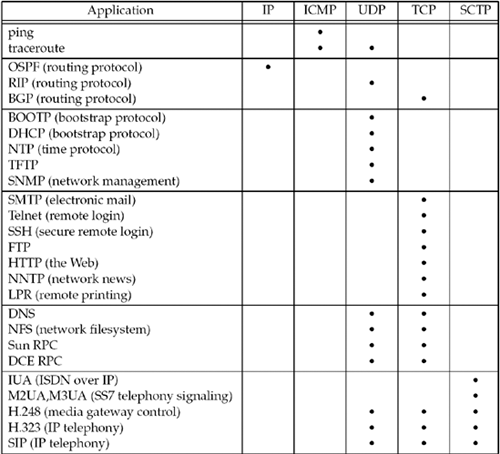
\includegraphics[height=6cm]{figs/02fig19.png}
  \end{center}
\end{frame}

\begin{frame}
  \frametitle{UDP vs TCP vs SCTP}
  \begin{center}
  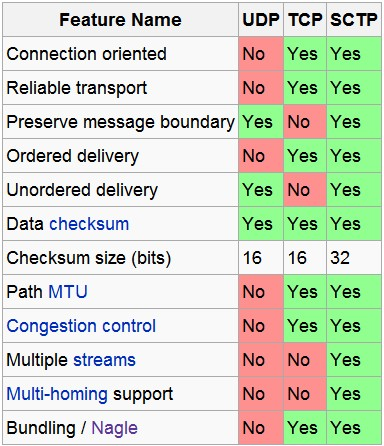
\includegraphics[height=6cm]{figs/udp-tcp-sctp-comparison.png}
  \end{center}
\end{frame}

\end{document}
